% !TEX root = ../../ctfp-print.tex

\lettrine[lhang=0.17]{N}{ow that you know} what a functor is, and have seen a few examples, let's
see how we can build larger functors from smaller ones. In particular
it's interesting to see which type constructors (which correspond to
mappings between objects in a category) can be extended to functors
(which include mappings between morphisms).

\section{Bifunctors}

Since functors are morphisms in $\Cat$ (the category of categories),
a lot of intuitions about morphisms --- and functions in particular ---
apply to functors as well. For instance, just like you can have a
function of two arguments, you can have a functor of two arguments, or a
\newterm{bifunctor}. On objects, a bifunctor maps every pair of objects,
one from category $\cat{C}$, and one from category $\cat{D}$, to an object in category
$\cat{E}$. Notice that this is just saying that it's a mapping from a
\newterm{Cartesian product} of categories $\cat{C}\times{}\cat{D}$ to $\cat{E}$.

\begin{figure}[H]
\centering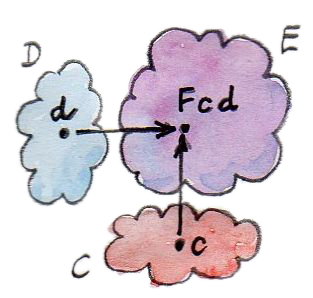
\includegraphics[width=0.3\textwidth]{images/bifunctor.jpg}
\end{figure}

\noindent
That's pretty straightforward. But functoriality means that a bifunctor
has to map morphisms as well. This time, though, it must map a pair of
morphisms, one from $\cat{C}$ and one from $\cat{D}$, to a morphism in $\cat{E}$.

Again, a pair of morphisms is just a single morphism in the product
category $\cat{C}\times{}\cat{D}$ to $\cat{E}$. We define a morphism in a Cartesian product of categories
as a pair of morphisms which goes from one pair of objects to another
pair of objects. These pairs of morphisms can be composed in the obvious
way:
\[(f, g) \circ (f', g') = (f \circ f', g \circ g')\]
The composition is associative and it has an identity --- a pair of
identity morphisms $(\id, \id)$. So a Cartesian product of categories
is indeed a category.

An easier way to think about bifunctors would be to consider them functors in
each argument separately. So instead of translating functorial laws ---
associativity and identity preservation --- from functors to bifunctors,
it would be enough to check them separately for each argument. However, in general,
separate functoriality is not enough to prove joint functoriality. Categories in which
joint functoriality fails are called \newterm{premonoidal}.

Let's define a bifunctor in Haskell. In this case all three categories
are the same: the category of Haskell types. A bifunctor is a type
constructor that takes two type arguments. Here's the definition of the
\code{Bifunctor} typeclass taken directly from the library
\code{Control.Bifunctor}:

\src{snippet01}

\begin{figure}[H]
\centering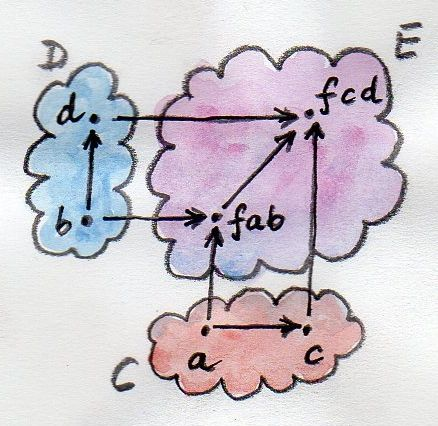
\includegraphics[width=0.3\textwidth]{images/bimap.jpg}
\caption{bimap}
\end{figure}

The type variable \code{f} represents the bifunctor. You can see that
in all type signatures it's always applied to two type arguments. The
first type signature defines \code{bimap}: a mapping of two functions
at once. The result is a lifted function,
\code{(f a b -> f c d)}, operating on types
generated by the bifunctor's type constructor. There is a default
implementation of \code{bimap} in terms of \code{first} and
\code{second}. (As mentioned before, this doesn't always work, because
the two maps may not commute, that is \code{first g . second h} may not
be the same as \code{second h . first g}.)


\noindent
The two other type signatures, \code{first} and \code{second}, are
the two \code{fmap}s witnessing the functoriality of \code{f} in the
first and the second argument, respectively.

\begin{figure}[H]
  \centering
  \begin{minipage}{0.45\textwidth}
      \centering
      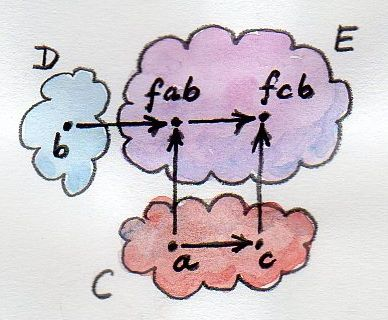
\includegraphics[width=0.65\textwidth]{images/first.jpg} % first figure itself
      \caption{first}
  \end{minipage}\hfill
  \begin{minipage}{0.45\textwidth}
      \centering
      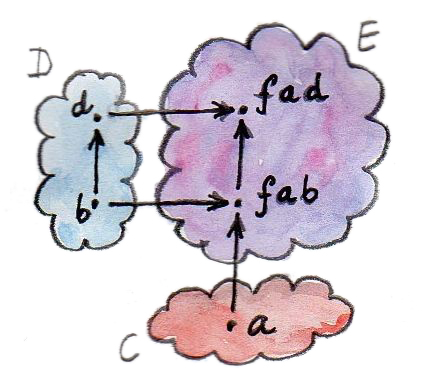
\includegraphics[width=0.6\textwidth]{images/second.jpg} % second figure itself
      \caption{second}
  \end{minipage}
\end{figure}

\noindent
The typeclass definition provides default implementations for both of
them in terms of \code{bimap}.

When declaring an instance of \code{Bifunctor}, you have a choice of
either implementing \code{bimap} and accepting the defaults for
\code{first} and \code{second}, or implementing both \code{first}
and \code{second} and accepting the default for \code{bimap} (of
course, you may implement all three of them, but then it's up to you to
make sure they are related to each other in this manner).

\section{Product and Coproduct Bifunctors}

An important example of a bifunctor is the categorical product --- a
product of two objects that is defined by a \hyperref[products-and-coproducts]{universal
construction}. If the product exists for any pair of objects, the
mapping from those objects to the product is bifunctorial. This is true
in general, and in Haskell in particular. Here's the \code{Bifunctor}
instance for a pair constructor --- the simplest product type:

\src{snippet02}[b]
There isn't much choice: \code{bimap} simply applies the first
function to the first component, and the second function to the second
component of a pair. The code pretty much writes itself, given the
types:

\src{snippet03}
The action of the bifunctor here is to make pairs of types, for
instance:

\begin{snip}{haskell}
(,) a b = (a, b)
\end{snip}
By duality, a coproduct, if it's defined for every pair of objects in a
category, is also a bifunctor. In Haskell, this is exemplified by the
\code{Either} type constructor being an instance of
\code{Bifunctor}:

\src{snippet04}[b]
This code also writes itself.

Now, remember when we talked about monoidal categories? A monoidal
category defines a binary operator acting on objects, together with a
unit object. I mentioned that $\Set$ is a monoidal category with
respect to Cartesian product, with the singleton set as a unit. And it's
also a monoidal category with respect to disjoint union, with the empty
set as a unit. What I haven't mentioned is that one of the requirements
for a monoidal category is that the binary operator be a bifunctor. This
is a very important requirement --- we want the monoidal product to be
compatible with the structure of the category, which is defined by
morphisms. We are now one step closer to the full definition of a
monoidal category (we still need to learn about naturality, before we
can get there).

\section{Functorial Algebraic Data Types}

We've seen several examples of parameterized data types that turned out
to be functors --- we were able to define \code{fmap} for them.
Complex data types are constructed from simpler data types. In
particular, algebraic data types (\acronym{ADT}s) are created using sums and
products. We have just seen that sums and products are functorial. We
also know that functors compose. So if we can show that the basic
building blocks of \acronym{ADT}s are functorial, we'll know that parameterized
\acronym{ADT}s are functorial too.

So what are the building blocks of parameterized algebraic data types?
First, there are the items that have no dependency on the type parameter
of the functor, like \code{Nothing} in \code{Maybe}, or \code{Nil}
in \code{List}. They are equivalent to the \code{Const} functor.
Remember, the \code{Const} functor ignores its type parameter (really,
the \emph{second} type parameter, which is the one of interest to us,
the first one being kept constant).

Then there are the elements that simply encapsulate the type parameter
itself, like \code{Just} in \code{Maybe}. They are equivalent to the
identity functor. I mentioned the identity functor previously, as the
identity morphism in \emph{Cat}, but didn't give its definition in
Haskell. Here it is:

\src{snippet05}

\src{snippet06}
You can think of \code{Identity} as the simplest possible container
that always stores just one (immutable) value of type \code{a}.

Everything else in algebraic data structures is constructed from these
two primitives using products and sums.

With this new knowledge, let's have a fresh look at the \code{Maybe}
type constructor:

\src{snippet07}
It's a sum of two types, and we now know that the sum is functorial. The
first part, \code{Nothing} can be represented as a \code{Const ()}
acting on \code{a} (the first type parameter of \code{Const} is set
to unit --- later we'll see more interesting uses of \code{Const}).
The second part is just a different name for the identity functor. We
could have defined \code{Maybe}, up to isomorphism, as:

\src{snippet08}
So \code{Maybe} is the composition of the bifunctor \code{Either}
with two functors, \code{Const ()} and \code{Identity}.
(\code{Const} is really a bifunctor, but here we always use it
partially applied.)

We've already seen that a composition of functors is a functor --- we
can easily convince ourselves that the same is true of bifunctors. All
we need is to figure out how a composition of a bifunctor with two
functors works on morphisms. Given two morphisms, we simply lift one
with one functor and the other with the other functor. We then lift the
resulting pair of lifted morphisms with the bifunctor.

We can express this composition in Haskell. Let's define a data type
that is parameterized by a bifunctor \code{bf} (it's a type variable
that is a type constructor that takes two types as arguments), two
functors \code{fu} and \code{gu} (type constructors that take one
type variable each), and two regular types \code{a} and \code{b}. We
apply \code{fu} to \code{a} and \code{gu} to \code{b}, and then
apply \code{bf} to the resulting two types:

\src{snippet09}
That's the composition on objects, or types. Notice how in Haskell we
apply type constructors to types, just like we apply functions to
arguments. The syntax is the same.

If you're getting a little lost, try applying \code{BiComp} to
\code{Either}, \code{Const ()}, \code{Identity}, \code{a}, and
\code{b}, in this order. You will recover our bare-bone version of
\code{Maybe b} (\code{a} is ignored).

The new data type \code{BiComp} is a bifunctor in \code{a} and
\code{b}, but only if \code{bf} is itself a \code{Bifunctor} and
\code{fu} and \code{gu} are \code{Functor}s. The compiler must
know that there will be a definition of \code{bimap} available for
\code{bf}, and definitions of \code{fmap} for \code{fu} and
\code{gu}. In Haskell, this is expressed as a precondition in the
instance declaration: a set of class constraints followed by a double
arrow:

\src{snippet10}[b]
The implementation of \code{bimap} for \code{BiComp} is given in
terms of \code{bimap} for \code{bf} and the two \code{fmap}s for
\code{fu} and \code{gu}. The compiler automatically infers all the
types and picks the correct overloaded functions whenever
\code{BiComp} is used.

The \code{x} in the definition of \code{bimap} has the type:

\src{snippet11}
which is quite a mouthful. The outer \code{bimap} breaks through the
outer \code{bf} layer, and the two \code{fmap}s dig under
\code{fu} and \code{gu}, respectively. If the types of \code{f1}
and \code{f2} are:

\src{snippet12}
then the final result is of the type
\code{bf (fu a') (gu b')}:

\src{snippet13}[b]
If you like jigsaw puzzles, these kinds of type manipulations can
provide hours of entertainment.

So it turns out that we didn't have to prove that \code{Maybe} was a
functor --- this fact followed from the way it was constructed as a sum
of two functorial primitives.

A perceptive reader might ask the question: If the derivation of the
\code{Functor} instance for algebraic data types is so mechanical,
can't it be automated and performed by the compiler? Indeed, it can, and
it is. You need to enable a particular Haskell extension by including
this line at the top of your source file:

\begin{snip}{haskell}
{-# LANGUAGE DeriveFunctor #-}
\end{snip}
and then add \code{deriving Functor} to your data structure:

\begin{snip}{haskell}
data Maybe a = Nothing | Just a deriving Functor
\end{snip}
and the corresponding \code{fmap} will be implemented for you.

The regularity of algebraic data structures makes it possible to derive
instances not only of \code{Functor} but of several other type
classes, including the \code{Eq} type class I mentioned before. There
is also the option of teaching the compiler to derive instances of your
own typeclasses, but that's a bit more advanced. The idea though is the
same: You provide the behavior for the basic building blocks and sums
and products, and let the compiler figure out the rest.

\section{Functors in C++}

If you are a C++ programmer, you obviously are on your own as far as
implementing functors goes. However, you should be able to recognize
some types of algebraic data structures in C++. If such a data structure
is made into a generic template, you should be able to quickly implement
\code{fmap} for it.

Let's have a look at a tree data structure, which we would define in
Haskell as a recursive sum type:

\src{snippet14}
As I mentioned before, one way of implementing sum types in C++ is
through class hierarchies. It would be natural, in an object-oriented
language, to implement \code{fmap} as a virtual function of the base
class \code{Functor} and then override it in all subclasses.
Unfortunately this is impossible because \code{fmap} is a template,
parameterized not only by the type of the object it's acting upon (the
\code{this} pointer) but also by the return type of the function
that's been applied to it. Virtual functions cannot be templatized in
C++. We'll implement \code{fmap} as a generic free function, and we'll
replace pattern matching with \code{dynamic\_cast}.

The base class must define at least one virtual function in order to
support dynamic casting, so we'll make the destructor virtual (which is
a good idea in any case):

\begin{snip}{cpp}
template<class T>
struct Tree { 
    virtual ~Tree() {};
};
\end{snip}
The \code{Leaf} is just an \code{Identity} functor in disguise:

\begin{snip}{cpp}
template<class T>
struct Leaf : public Tree<T> {
    T _label;
    Leaf(T l) : _label(l) {}
};
\end{snip}
The \code{Node} is a product type:

\begin{snip}{cpp}
template<class T>
struct Node : public Tree<T> {
    Tree<T> * _left;
    Tree<T> * _right;
    Node(Tree<T> * l, Tree<T> * r) : _left(l), _right(r) {}
};
\end{snip}
When implementing \code{fmap} we take advantage of dynamic dispatching
on the type of the \code{Tree}. The \code{Leaf} case applies the
\code{Identity} version of \code{fmap}, and the \code{Node} case
is treated like a bifunctor composed with two copies of the
\code{Tree} functor. As a C++ programmer, you're probably not used to
analyzing code in these terms, but it's a good exercise in categorical
thinking.

\begin{snip}{cpp}
template<class A, class B>
Tree<B> * fmap(std::function<B(A)> f, Tree<A> * t) {
    Leaf<A> * pl = dynamic_cast <Leaf<A>*>(t);
    if (pl)
        return new Leaf<B>(f (pl->_label));
    Node<A> * pn = dynamic_cast<Node<A>*>(t);
    if (pn)
        return new Node<B>( fmap<A>(f, pn->_left) 
                          , fmap<A>(f, pn->_right));
    return nullptr;
}
\end{snip}
For simplicity, I decided to ignore memory and resource management
issues, but in production code you would probably use smart pointers
(unique or shared, depending on your policy).

Compare it with the Haskell implementation of \code{fmap}:

\src{snippet15}
This implementation can also be automatically derived by the compiler.

\section{The Writer Functor}

I promised that I would come back to the \hyperref[kleisli-categories]{Kleisli
category} I described earlier. Morphisms in that category were
represented as ``embellished'' functions returning the \code{Writer}
data structure.

\src{snippet16}
I said that the embellishment was somehow related to endofunctors. And,
indeed, the \code{Writer} type constructor is functorial in
\code{a}. We don't even have to implement \code{fmap} for it,
because it's just a simple product type.

But what's the relation between a Kleisli category and a functor --- in
general? A Kleisli category, being a category, defines composition and
identity. Let me remind you that the composition is given by the fish
operator:

\src{snippet17}
and the identity morphism by a function called \code{return}:

\src{snippet18}
It turns out that, if you look at the types of these two functions long
enough (and I mean, \emph{long} enough), you can find a way to combine
them to produce a function with the right type signature to serve as
\code{fmap}. Like this:

\src{snippet19}
Here, the fish operator combines two functions: one of them is the
familiar \code{id}, and the other is a lambda that applies
\code{return} to the result of acting with \code{f} on the lambda's
argument. The hardest part to wrap your brain around is probably the use
of \code{id}. Isn't the argument to the fish operator supposed to be a
function that takes a ``normal'' type and returns an embellished type?
Well, not really. Nobody says that \code{a} in
\code{a -> Writer b} must be a ``normal'' type. It's a
type variable, so it can be anything, in particular it can be an
embellished type, like \code{Writer b}.

So \code{id} will take \code{Writer a} and turn it into
\code{Writer a}. The fish operator will fish out the value of
\code{a} and pass it as \code{x} to the lambda. There, \code{f}
will turn it into a \code{b} and \code{return} will embellish it,
making it \code{Writer b}. Putting it all together, we end up with a
function that takes \code{Writer a} and returns \code{Writer b},
exactly what \code{fmap} is supposed to produce.

Notice that this argument is very general: you can replace
\code{Writer} with any type constructor. As long as it supports a fish
operator and \code{return}, you can define \code{fmap} as well. So
the embellishment in the Kleisli category is always a functor. (Not
every functor, though, gives rise to a Kleisli category.)

You might wonder if the \code{fmap} we have just defined is the same
\code{fmap} the compiler would have derived for us with
\code{deriving Functor}. Interestingly enough, it is. This is due to
the way Haskell implements polymorphic functions. It's called
\newterm{parametric polymorphism}, and it's a source of so called
\newterm{theorems for free}. One of those theorems says that, if there is
an implementation of \code{fmap} for a given type constructor, one
that preserves identity, then it must be unique.

\section{Covariant and Contravariant Functors}

Now that we've reviewed the writer functor, let's go back to the reader
functor. It was based on the partially applied function-arrow type
constructor:

\src{snippet20}
We can rewrite it as a type synonym:

\src{snippet21}
for which the \code{Functor} instance, as we've seen before, reads:

\src{snippet22}
But just like the pair type constructor, or the \code{Either} type
constructor, the function type constructor takes two type arguments. The
pair and \code{Either} were functorial in both arguments --- they were
bifunctors. Is the function constructor a bifunctor too?

Let's try to make it functorial in the first argument. We'll start with
a type synonym --- it's just like the \code{Reader} but with the
arguments flipped:

\src{snippet23}
This time we fix the return type, \code{r}, and vary the argument
type, \code{a}. Let's see if we can somehow match the types in order
to implement \code{fmap}, which would have the following type
signature:

\src{snippet24}
With just two functions taking \code{a} and returning, respectively,
\code{b} and \code{r}, there is simply no way to build a function
taking \code{b} and returning \code{r}! It would be different if we
could somehow invert the first function, so that it took \code{b} and
returned \code{a} instead. We can't invert an arbitrary function, but
we can go to the opposite category.

A short recap: For every category $\cat{C}$ there is a dual category
$\cat{C}^{op}$. It's a category with the same objects as
$\cat{C}$, but with all the arrows reversed.

Consider a functor that goes between $\cat{C}^{op}$ and
some other category $\cat{D}$:
\[F \Colon \cat{C}^{op} \to \cat{D}\]
Such a functor maps a morphism $f^{op} \Colon a \to b$ in
$\cat{C}^{op}$ to the morphism $F f^{op} \Colon F a \to F b$ in $\cat{D}$. But the morphism
$f^{op}$ secretly corresponds to some morphism
$f \Colon b \to a$ in the original category $\cat{C}$. Notice the
inversion.

Now, $F$ is a regular functor, but there is another mapping we can
define based on $F$, which is not a functor --- let's call it
$G$. It's a mapping from $\cat{C}$ to $\cat{D}$. It maps objects the
same way $F$ does, but when it comes to mapping morphisms, it
reverses them. It takes a morphism $f \Colon b \to a$ in $\cat{C}$, maps
it first to the opposite morphism $f^{op} \Colon a \to b$
and then uses the functor $F$ on it, to get $F f^{op} \Colon F\ a \to F\ b$.

Considering that $F a$ is the same as $G a$ and $F b$ is
the same as $G b$, the whole trip can be described as: $G f \Colon (b \to a) \to (G a \to G b)$
It's a ``functor with a twist.'' A mapping of categories that inverts
the direction of morphisms in this manner is called a
\emph{contravariant functor}. Notice that a contravariant functor is
just a regular functor from the opposite category. The regular functors,
by the way --- the kind we've been studying thus far --- are called
\emph{covariant} functors.

\begin{figure}[H]
\centering
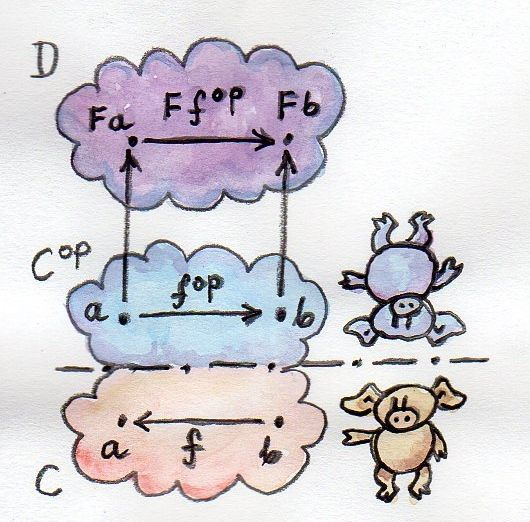
\includegraphics[width=40mm]{images/contravariant.jpg}
\end{figure}

\noindent
Here's the typeclass defining a contravariant functor (really, a
contravariant \emph{endo}functor) in Haskell:

\src{snippet25}
Our type constructor \code{Op} is an instance of it:

\src{snippet26}
Notice that the function \code{f} inserts itself \emph{before} (that
is, to the right of) the contents of \code{Op} --- the function
\code{g}.

The definition of \code{contramap} for \code{Op} may be made even
terser, if you notice that it's just the function composition operator
with the arguments flipped. There is a special function for flipping
arguments, called \code{flip}:

\src{snippet27}
With it, we get:

\src{snippet28}

\section{Profunctors}

We've seen that the function-arrow operator is contravariant in its
first argument and covariant in the second. Is there a name for such a
beast? It turns out that, if the target category is $\Set$, such a
beast is called a \newterm{profunctor}. Because a contravariant functor is
equivalent to a covariant functor from the opposite category, a
profunctor is defined as:
\[\cat{C}^{op} \times \cat{D} \to \Set\]
Since, to first approximation, Haskell types are sets, we apply the name
\code{Profunctor} to a type constructor \code{p} of two arguments,
which is contra-functorial in the first argument and functorial in the
second. Here's the appropriate typeclass taken from the
\code{Data.Profunctor} library:

\src{snippet29}[b]
All three functions come with default implementations. Just like with
\code{Bifunctor}, when declaring an instance of \code{Profunctor},
you have a choice of either implementing \code{dimap} and accepting
the defaults for \code{lmap} and \code{rmap}, or implementing both
\code{lmap} and \code{rmap} and accepting the default for
\code{dimap}.

\begin{figure}[H]
\centering
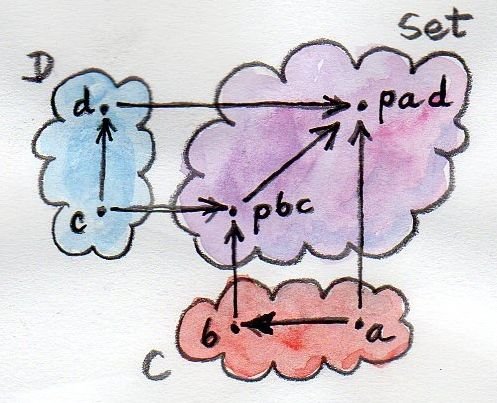
\includegraphics[width=0.4\textwidth]{images/dimap.jpg}
\caption{dimap}
\end{figure}

\noindent
Now we can assert that the function-arrow operator is an instance of a
\code{Profunctor}:

\src{snippet30}[b]
Profunctors have their application in the Haskell lens library. We'll
see them again when we talk about ends and coends.

\section{The Hom-Functor}

The above examples are the reflection of a more general statement that
the mapping that takes a pair of objects $a$ and $b$ and
assigns to it the set of morphisms between them, the hom-set
$\cat{C}(a, b)$, is a functor. It is a functor from the product
category $\cat{C}^{op}\times{}\cat{C}$ to the category of sets, $\Set$.

Let's define its action on morphisms. A morphism in
$\cat{C}^{op}\times{}\cat{C}$ is a pair of morphisms from $\cat{C}$:
\begin{gather*}
f \Colon a' \to a \\
g \Colon b \to b'
\end{gather*}
The lifting of this pair must be a morphism (a function) from the set
$\cat{C}(a, b)$ to the set $\cat{C}(a', b')$. Just pick
any element $h$ of $\cat{C}(a, b)$ (it's a morphism from
$a$ to $b$) and assign to it:
\[g \circ h \circ f\]
which is an element of $\cat{C}(a', b')$.

As you can see, the hom-functor is a special case of a profunctor.

\section{Challenges}

\begin{enumerate}
\tightlist
\item
  Show that the data type:

\begin{snip}{haskell}
data Pair a b = Pair a b
\end{snip}

  is a bifunctor. For additional credit implement all three methods of
  \code{Bifunctor} and use equational reasoning to show that these
  definitions are compatible with the default implementations whenever
  they can be applied.
\item
  Show the isomorphism between the standard definition of \code{Maybe}
  and this desugaring:

\begin{snip}{haskell}
type Maybe' a = Either (Const () a) (Identity a)
\end{snip}

  Hint: Define two mappings between the two implementations. For
  additional credit, show that they are the inverse of each other using
  equational reasoning.
\item
  Let's try another data structure. I call it a \code{PreList} because
  it's a precursor to a \code{List}. It replaces recursion with a type
  parameter \code{b}.

\begin{snip}{haskell}
data PreList a b = Nil | Cons a b
\end{snip}

  You could recover our earlier definition of a \code{List} by
  recursively applying \code{PreList} to itself (we'll see how it's
  done when we talk about fixed points).

  Show that \code{PreList} is an instance of \code{Bifunctor}.
\item
  Show that the following data types define bifunctors in \code{a} and
  \code{b}:

\begin{snip}{haskell}
data K2 c a b = K2 c

data Fst a b = Fst a

data Snd a b = Snd b
\end{snip}

  For additional credit, check your solutions against Conor McBride's
  paper \urlref{http://strictlypositive.org/CJ.pdf}{Clowns to the Left of
  me, Jokers to the Right}.
\item
  Define a bifunctor in a language other than Haskell. Implement
  \code{bimap} for a generic pair in that language.
\item
  Should \code{std::map} be considered a bifunctor or a profunctor in
  the two template arguments \code{Key} and \code{T}? How would you
  redesign this data type to make it so?
\end{enumerate}
